\subsection{Analysis of Distance Estimates}

\subsubsection{Model / Manual Distance Comparison}\label{subsubsec:distance_comparison}

In this section, the precision and accuracy of the distance estimates generated using the
four configurations of the distance estimation pipeline (outlined in
Section~\ref{subsubsec:configuratons}) are evaluated.
In order for these data to be analysed, the estimates are benchmarked against their
corresponding manual distance estimates (supplied with the dataset), thus these estimates
use detection frames originating from the manual sample (Section~\ref{subsubsec:sampling}).

Ideally, each and every manual distance should be joined to its corresponding modelled
distance estimate; however, due to the absence of any frame-position data associated
with the manual annotations, automating this using traditional algorithms is impossible
in circumstances where multiple chimps are captured in a single frame.
This is because when multiple individuals are detected, there is ambiguity in regard to
which distance a given modelled distance should be joined to.
Moreover, approaching this task manually is extremely labour-intensive and was therefore
outside the scope of this project.
As a result, this analysis focuses on distance comparisons associated with frames capturing
only a single individual.

Upon joining the modelled distance estimates to their corresponding manual estimates, the
overall errors of each of the four pipeline configurations were calculated.
Table~\ref{tab:overall_errors} shows the mean average error, root mean squared error,
average difference (i.e., mean($model_i$ - $manual_i$)) and the result of a statistical
difference test (i.e., where p-value < 0.05).
To note, while both the mean average and root mean squared errors give a measure of the
absolute error of the configurations, the average difference does not and is affected by
cancellation between overestimates and underestimates.
Therefore, it is used as a metric to assess whether a given configuration over or
under-predicts relative to the manual distance estimation method, where a positive value
indicates over-prediction while a negative value indicates under-prediction.

The modelled distance estimates were then grouped by their corresponding manual estimates (i.e.,
0.5 m, 1.0 m, \ldots 15 m).
Figure~\ref{fig:distance_comparison} shows the averages of the modelled estimates for each
group while Figure~\ref{fig:spread_comparison} shows each individual modelled estimate for
each group, giving a visualisation of the spread of the estimates.
These individual errors for each of these groups were then calculated.
Figure~\ref{fig:mae} show the change in mean average error for each group while
Figure~\ref{fig:rmse} shows the change in root mean squared error for each group.

\vspace{1cm}

\begin{table}[htbp]
    \centering
    \caption{Mean average error (MAE), root mean squared error (RMSE), average difference between
    model and manual estimate ($\Delta_{average}$) and result of Wilcoxon signed rank test for
    statistical difference. These data describe all distance estimates for each pipeline
    configuration collectivelly.)}
    \label{tab:overall_errors}
    \begin{tabular}{ccccc}
        \textbf{Method} & \textbf{MAE / m} & \textbf{RMSE / m} & \textbf{$\Delta_{average}$ / m}
        & \textbf{Statistical Difference} \\
        \midrule
        DPT, BBOX & 1.81 & 2.66 & 0.586 & YES \\
        DPT, SEG  & 1.70 & 2.45 & 0.836 & YES \\
        DA, BBOX  & 2.03 & 2.62 & 1.49  & YES \\
        DA, SEG   & 3.00 & 3.52 & 2.80  & YES \\
    \end{tabular}
\end{table}

\clearpage

\begin{figure}[p]
    \centering
    \vspace{1cm}
    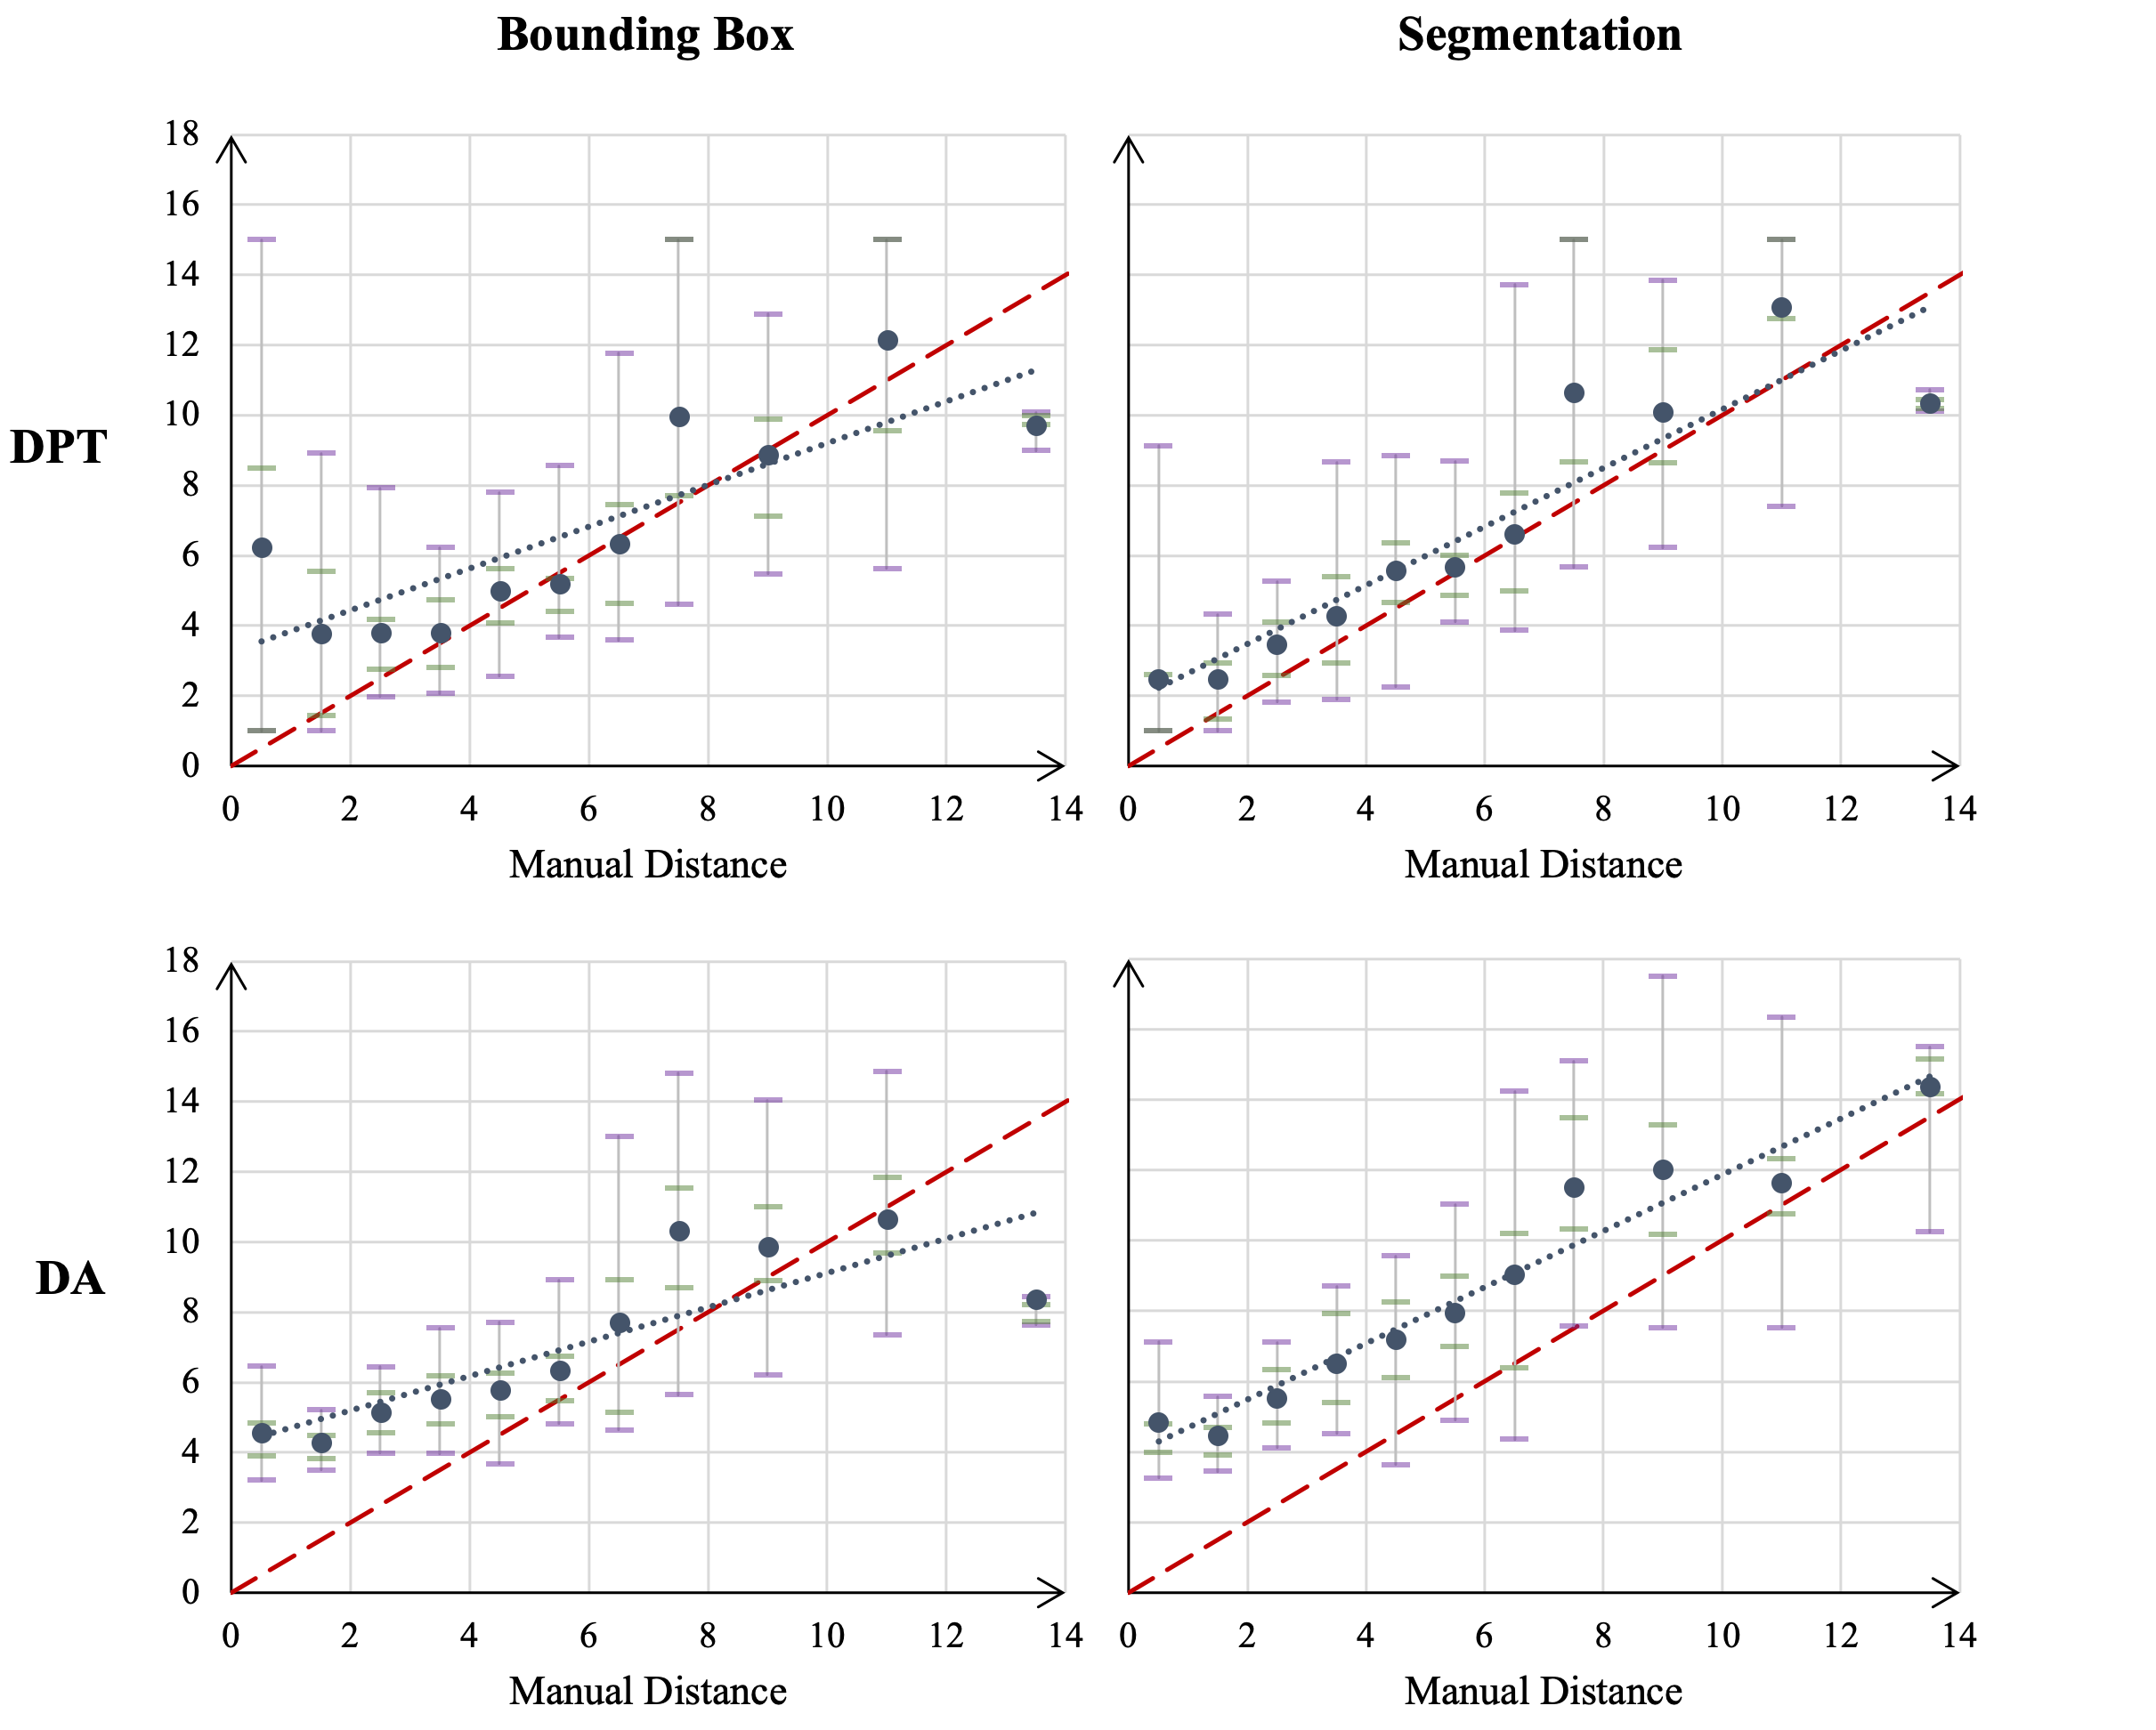
\includegraphics[width=1.01\textwidth]{body/analysis/assets/distance_graphs/averages}
    \caption{Graphs showing mean modelled distance estimates mapped to thier corresponding manual
    estimates for the configurations: DPT/bounding box (top-left), DPT/segmentation (top-right),
        DA/bounding box (bottom-left) and DA/segmentation (bottom-right). The blue dotted line
        shows the fitted regression line. The red dashed line shows the ideal (i.e., model=manual).
        the error bars show the 25–75 (green) and 5–95 (purple) percentiles.}
    \label{fig:distance_comparison}
\end{figure}

\begin{figure}[p]
    \centering
    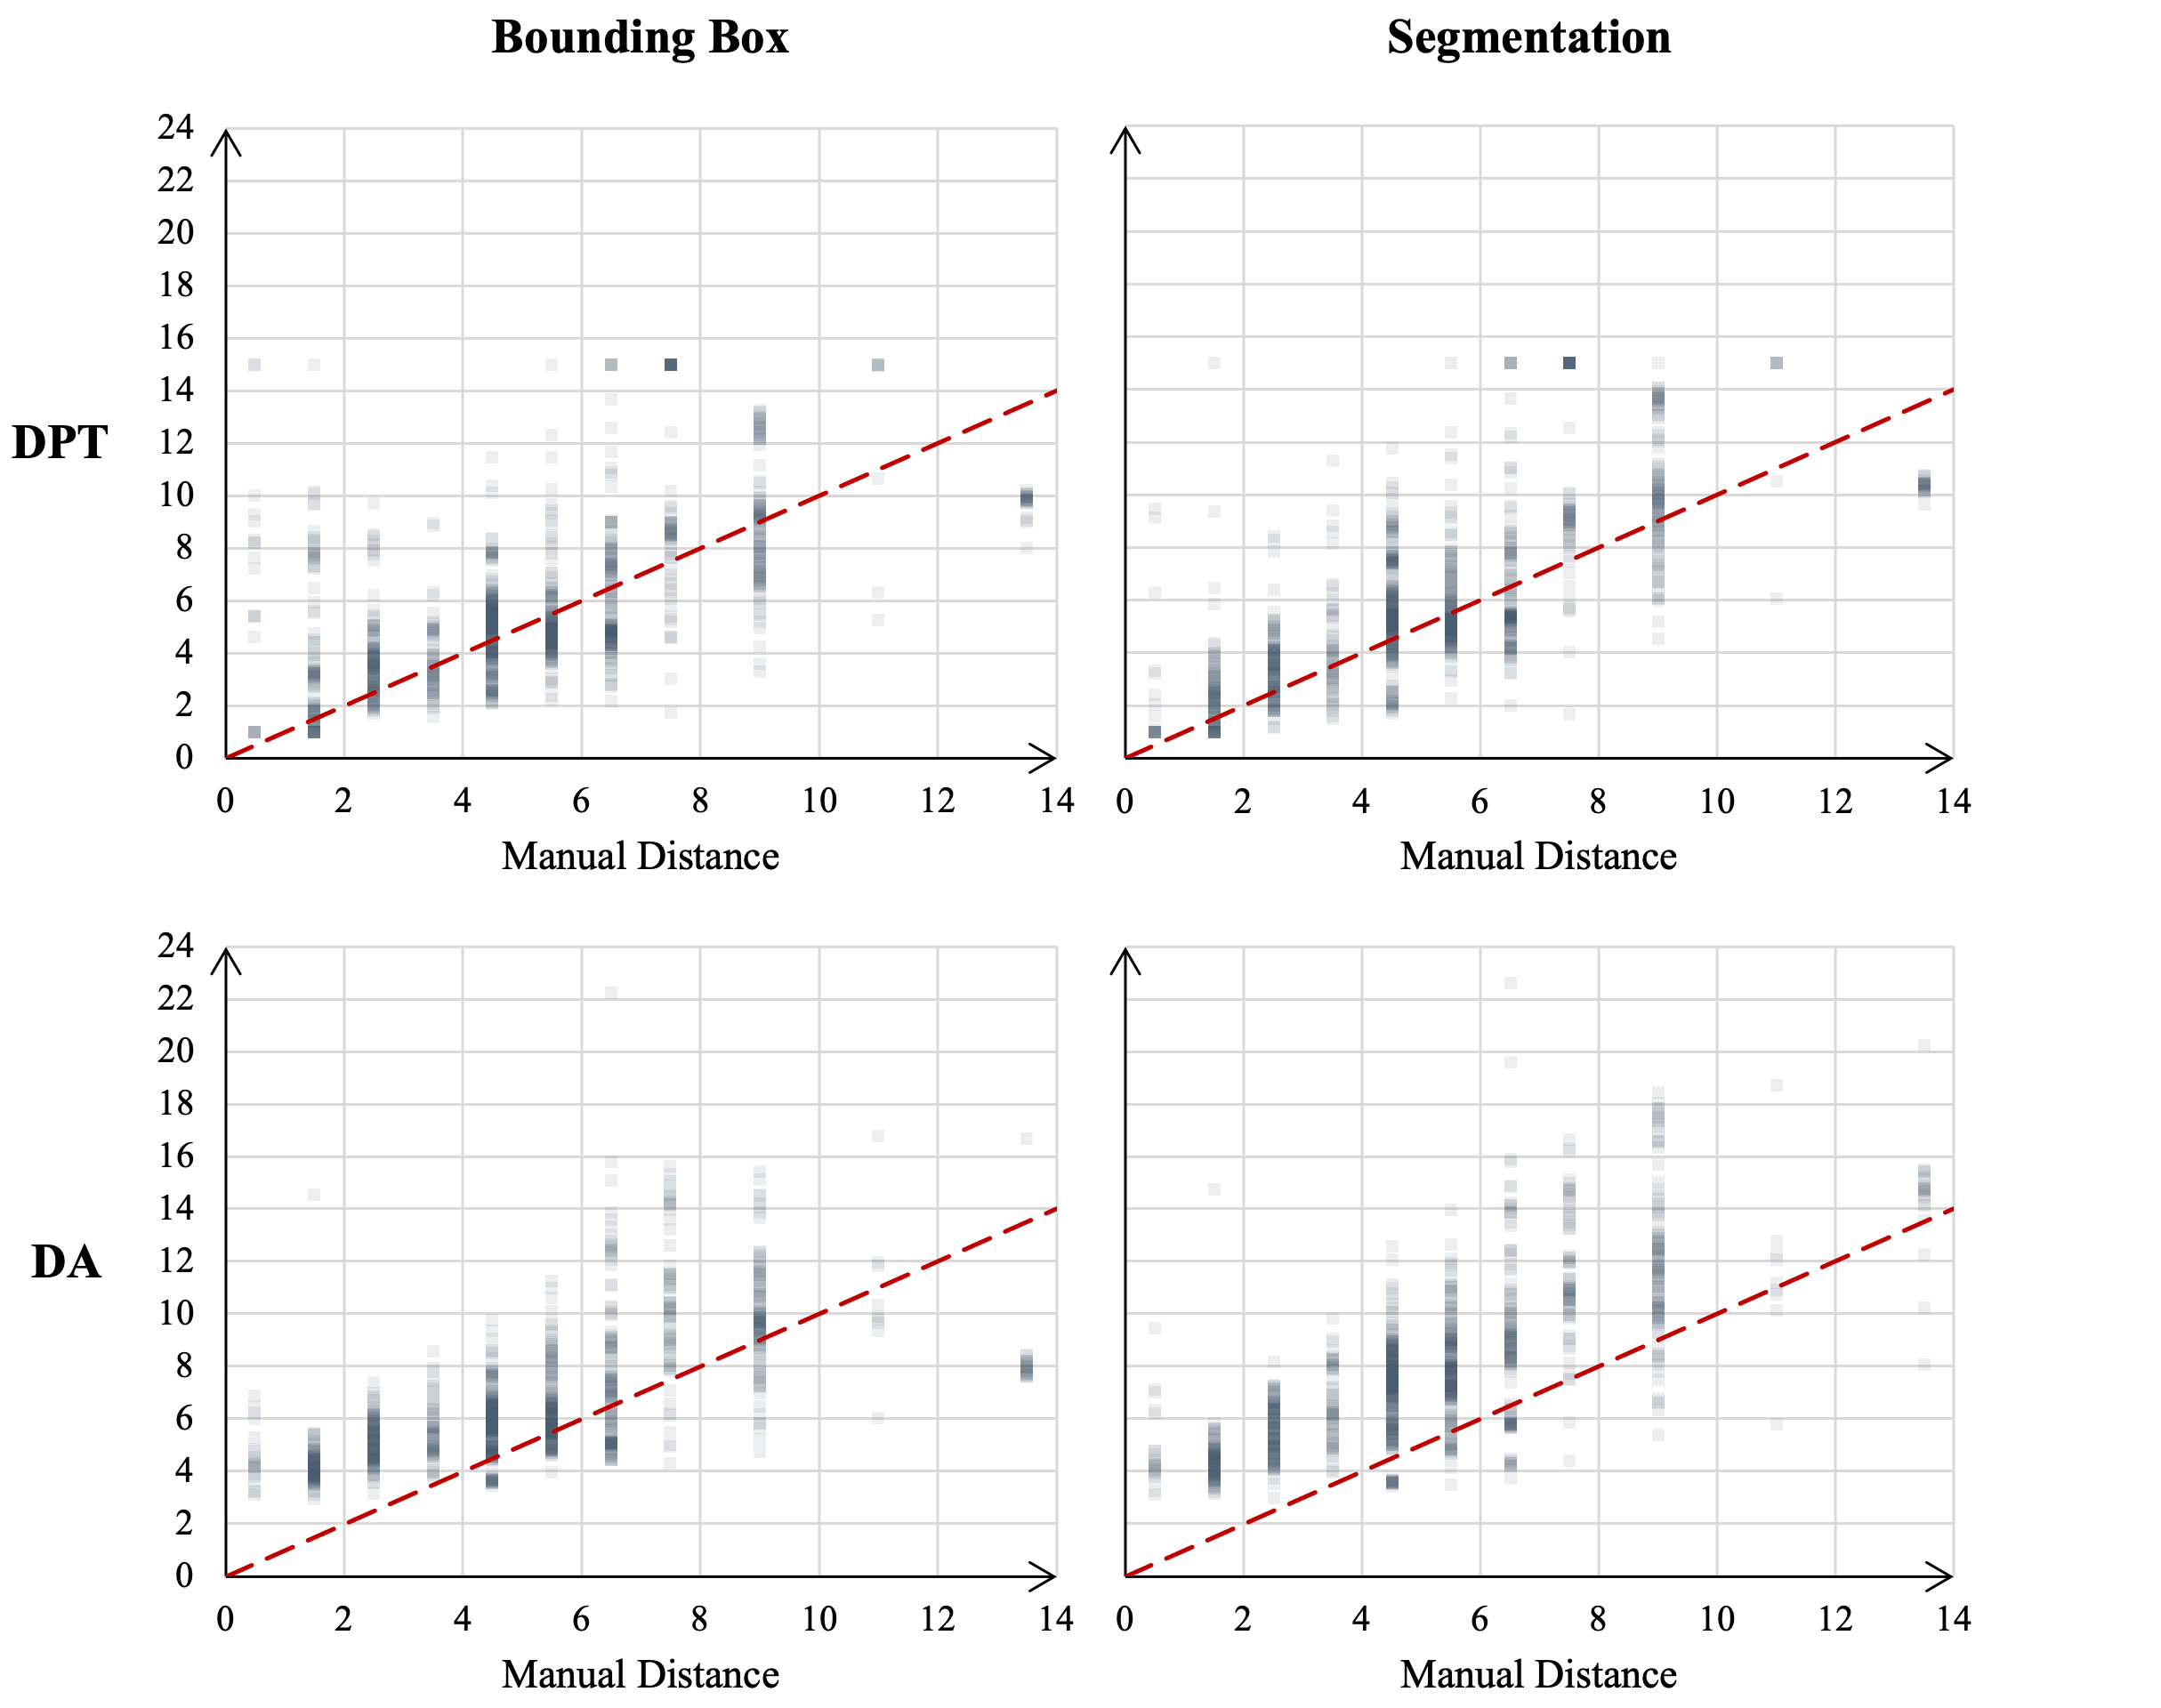
\includegraphics[width=1.01\textwidth]{body/analysis/assets/distance_graphs/spread}
    \caption{Graphs showing all modelled distance estimates mapped to thier corresponding manual
        estimates for the configurations: DPT/bounding box (top-left), DPT/segmentation (top-right),
        DA/bounding box (bottom-left) and DA/segmentation (bottom-right). The red dashed line shows
        the ideal (i.e., model=manual).}
    \label{fig:spread_comparison}
\end{figure}

\clearpage

%\subsubsection{Error Analysis}

\begin{figure}[H]
    \vspace{1cm}
    \centering
    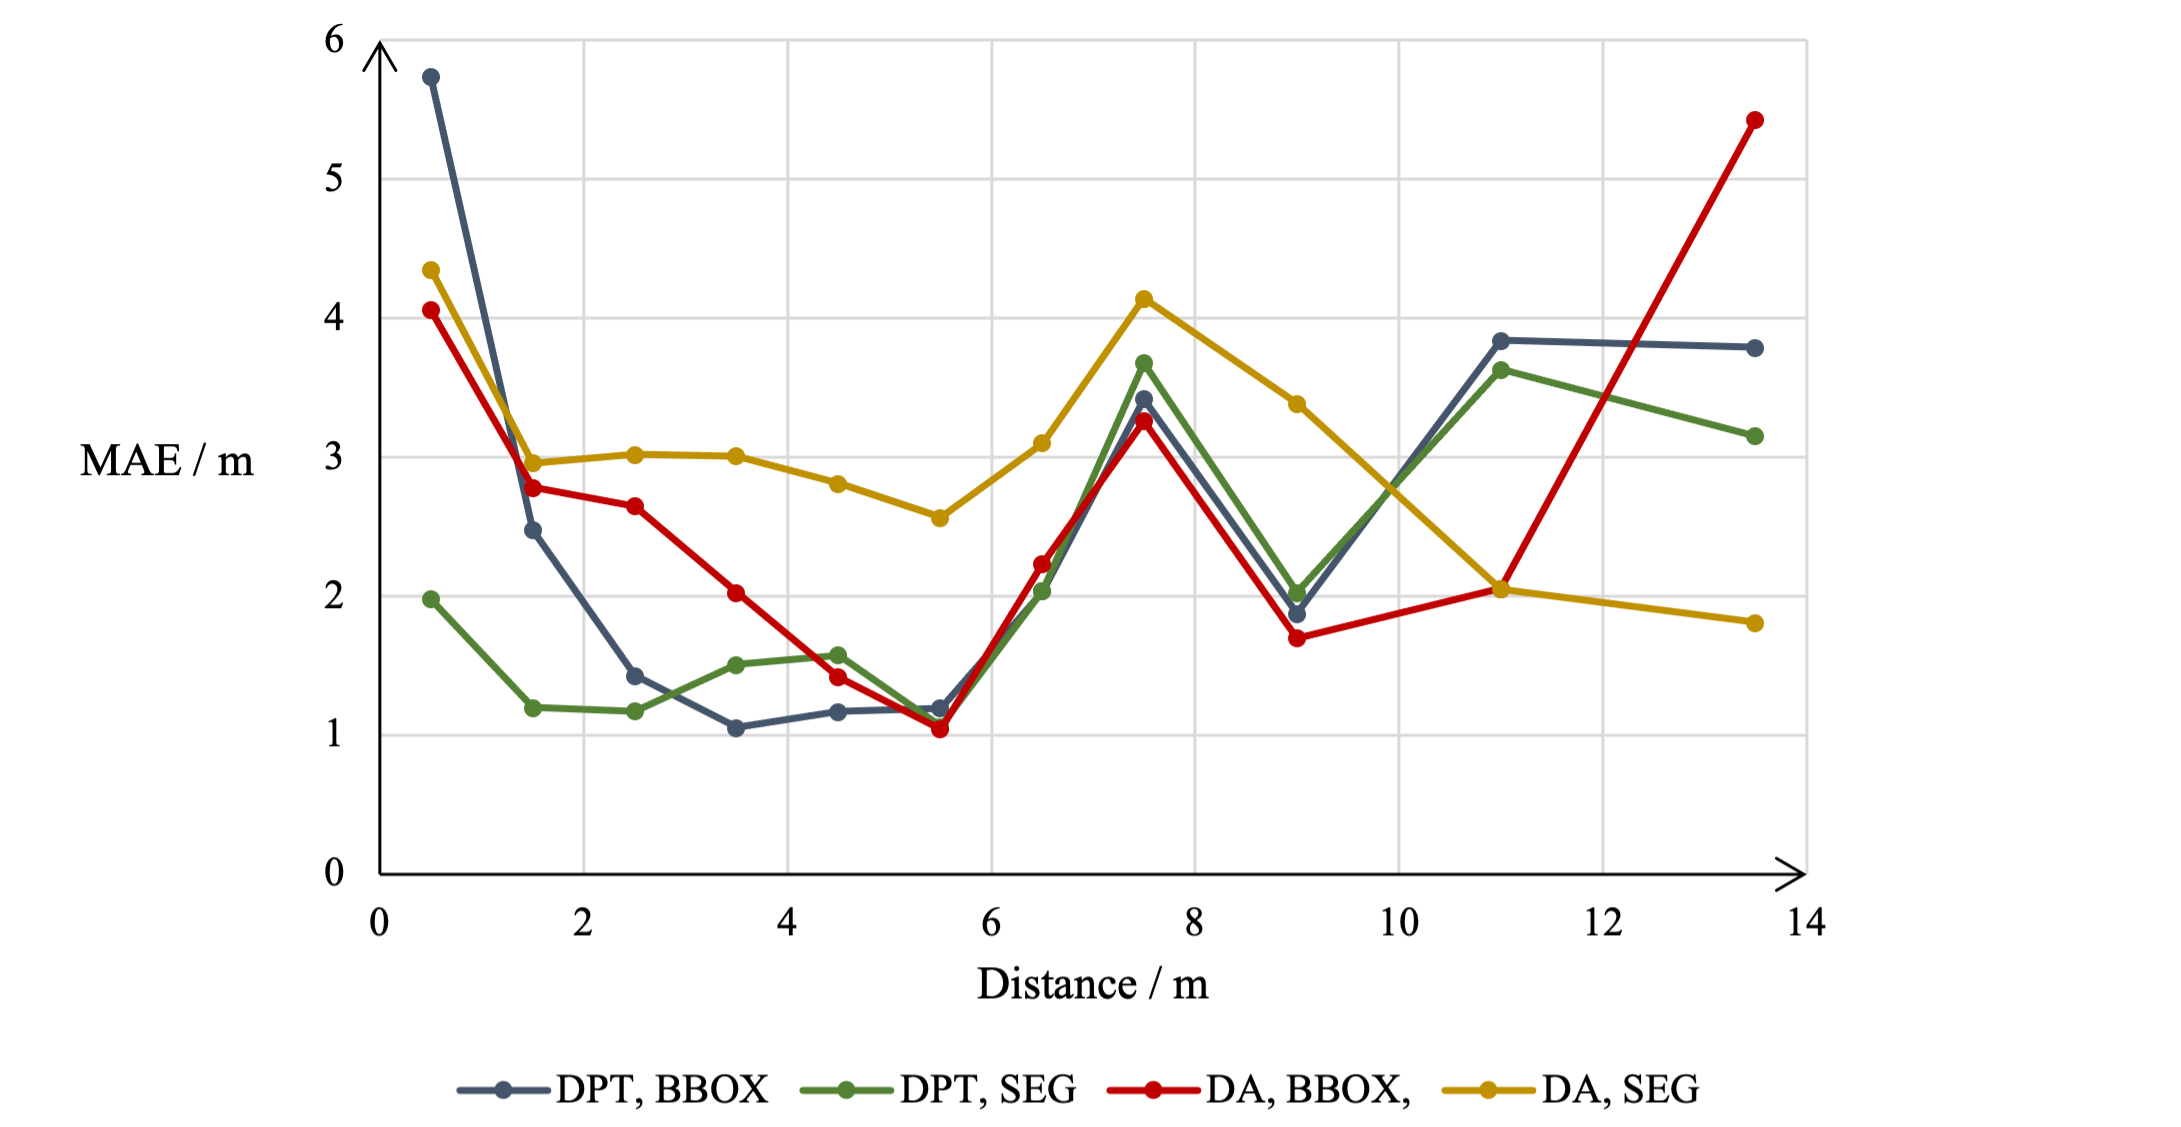
\includegraphics[width=1.01\textwidth]{body/analysis/assets/errors/MAE}
    \caption{Mean average error for distance estimates grouped by their corresponding manual
    estimates for each pipeline configuration.}
    \label{fig:mae}

    \vspace{2cm}

    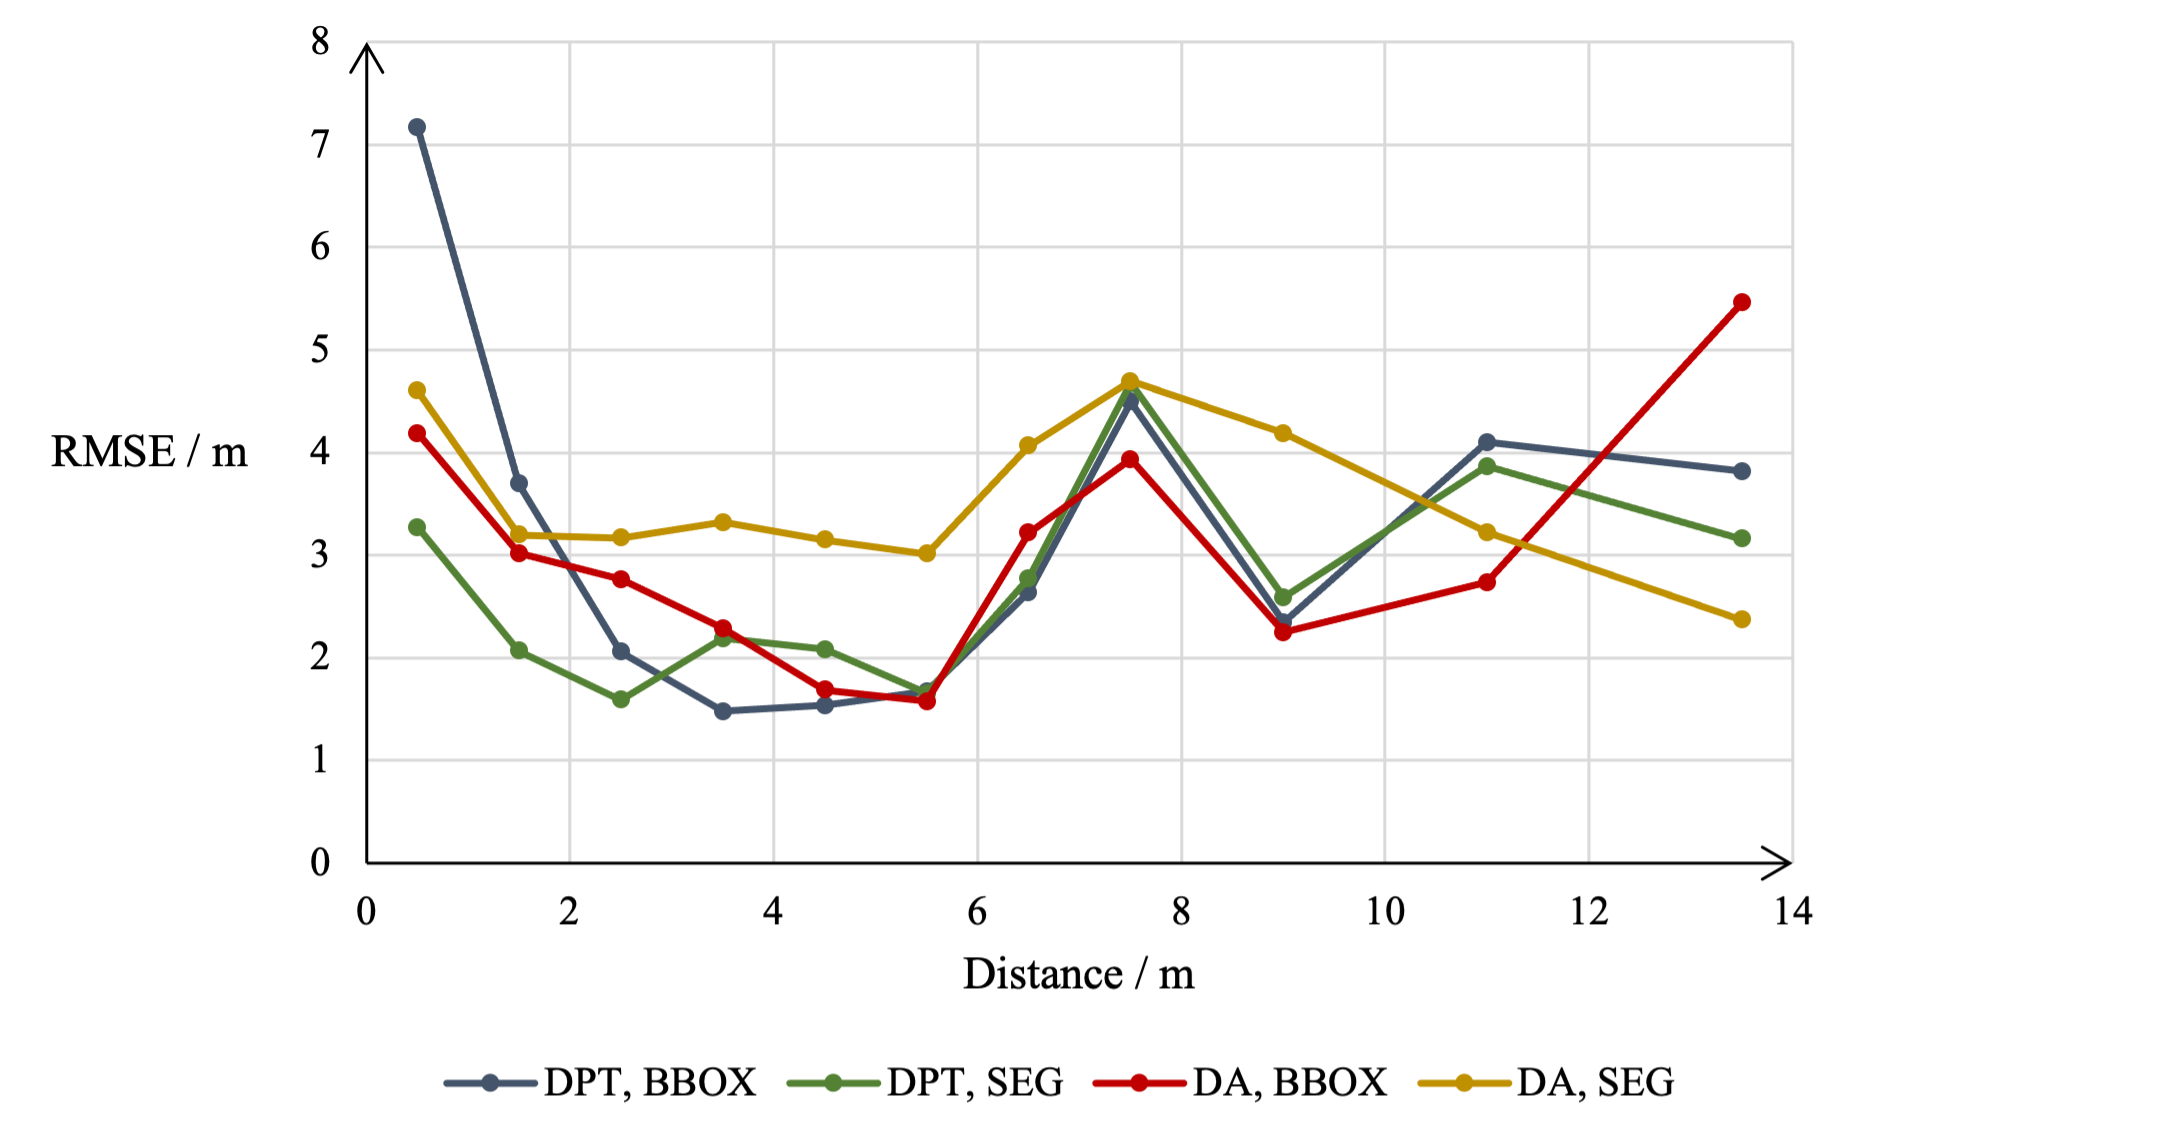
\includegraphics[width=1.01\textwidth]{body/analysis/assets/errors/RMSE}
    \caption{Root mean squared error for distance estimates grouped by their corresponding manual
    estimates for each pipeline configuration.}
    \label{fig:rmse}
\end{figure}

\clearpage

For all configurations, it is seen that there is a spread range of estimated distances
within the groups.
Contrasting the distance estimates of the two detection method using DPT distance estimation,
an increase in both accuracy and precision is observed for the segmentation method compared
to the bounding box method at close distances (i.e., < 2 meters).
For modelled distances corresponding to manual estimates of 0.5 meters, the bounding box
method gives a MAE of 5.74 meters, a RMSE of 7.17 meters and an interquartile range of 7.50
meters while the segmentation method gives a MAE of 1.98 meters, a RMSE of 3.27 meters and
and interquartile range of 1.61 meters.
This is explained by a better detection frame calibration alignment.
Here, only the detection frame pixels defined by the chimpanzee segmentation are masked as
opposed to those within the entire bounding box.
As a result, more pixels corresponding to the transect background which are common to both
the calibration and detection frames are available for depth scale alignment, leading to a
superior calibration of the detection frame depth scale.

\begin{figure}[htbp]
    \centering
    \makebox[0.8\textwidth][c]{
        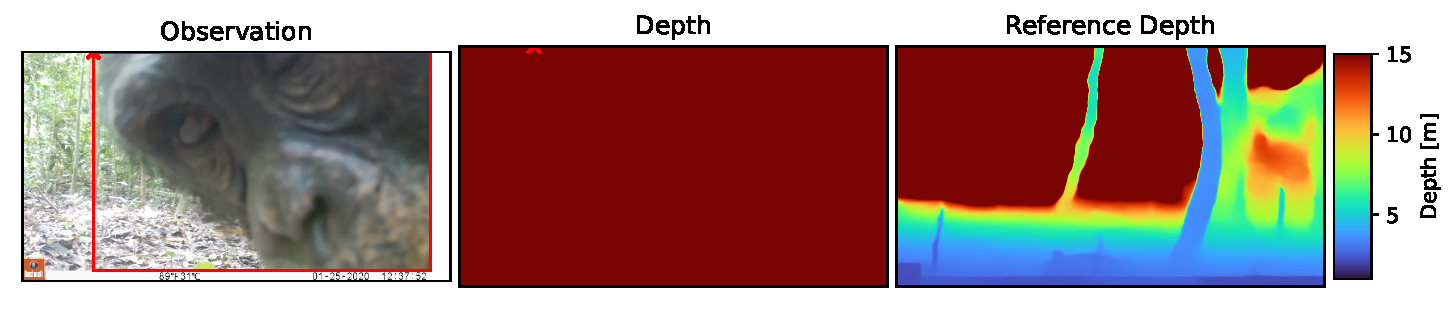
\includegraphics[width=0.9\textwidth]{body/analysis/assets/depth_maps/close_bbox}
    }\\[1mm]
    \makebox[0.8\textwidth][c]{
        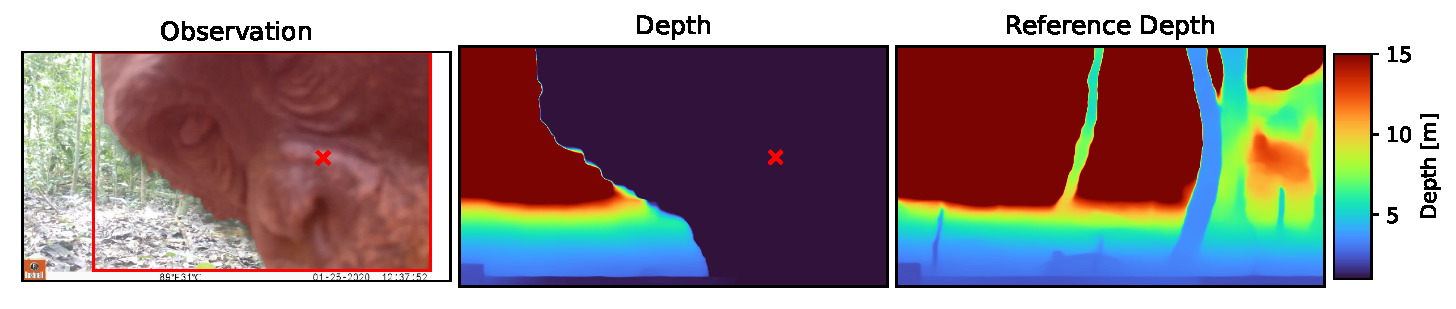
\includegraphics[width=0.9\textwidth]{body/analysis/assets/depth_maps/close_seg}
    }
    \caption{Example of DPT depth maps generated using bounding box (top) and segmentation
        (bottom) detection methods at a detection distance of 0.5 meters (manual estimate)}
    \label{fig:bbox_vs_seg_close}
\end{figure}

This effect is exemplified in Figure~\ref{fig:bbox_vs_seg_close}, where the bounding box
method results in an effectively failed calibration while the segmentation method succeeds.
In this example, the bounding box method estimates a distance of 15.0 meters whereas the
segmentation method estimates 1.0 meters.


\clearpage

\subsubsection{Qualitative Analysis}
depth map diagrams
close/far failure cases, sweet spot

\subsubsection{Effects of Varying Calibration}